\documentclass{article}
\usepackage{arxiv}

\usepackage[utf8]{inputenc}
\usepackage[english, russian]{babel}
\usepackage[T1]{fontenc}
\usepackage{url}
\usepackage{booktabs}
\usepackage{amsfonts}
\usepackage{nicefrac}
\usepackage{microtype}
\usepackage{lipsum}
\usepackage{graphicx}
\usepackage{natbib}
\usepackage{doi}



\title{Восстановление прогноза, сделанного в метрическом вероятностном пространстве, в исходное пространство (временных рядов)}

\author{ Maxim Divilkovskiy \\
% \thanks{Use footnote for providing further
% 		information about author (webpage, alternative
% 		address)---\emph{not} for acknowledging funding agencies.} \\
	Chair of Data Analysis\\
	MIPT\\
	divilkovskii.mm@phystech.edu \\
	%% examples of more authors
	\And
	Vadim Strijov \\
	FRC CSC of the RAS\\
	Moscow, Russia\\
        strijov@phystech.edu \\
	% Santa Narimana, Levand \\
	% \texttt{stariate@ee.mount-sheikh.edu} \\
	%% \AND
	%% Coauthor \\
	%% Affiliation \\
	%% Address \\
	%% \texttt{email} \\
	%% \And
	%% Coauthor \\
	%% Affiliation \\
	%% Address \\
	%% \texttt{email} \\
	%% \And
	%% Coauthor \\
	%% Affiliation \\
	%% Address \\
	%% \texttt{email} \\
}
\date{}

\renewcommand{\shorttitle}{\textit{arXiv} Template}

%%% Add PDF metadata to help others organize their library
%%% Once the PDF is generated, you can check the metadata with
%%% $ pdfinfo template.pdf
\hypersetup{
pdfauthor={Maxim Divilkovskiy},
}

\graphicspath{ {./figures/} }

\begin{document}
\maketitle

\begin{abstract}
	Исследование посвящено проблеме прогнозирования временных рядов с высокой ковариацией. Задача решается для наборов временных рядов с высокой дисперсией, проявляющейся, например, в сигналах головного мозга или ценах финансовых активов. Для решения данной задачи предлагается построение пространства парных расстояний, представляющего метрическую конфигурацию временных рядов. Прогноз осуществляется в этом пространстве, а затем результат возвращается в исходное пространство.
	В данной статье рассматриваются методы перевода прогноза из метрического пространства в исходное пространство временных рядов. Помимо этого, приводится оценка качества прогноза. Новизна работы заключается в использовании риманова пространства в качестве метрического, а также в использовании римановых моделей.


\end{abstract}


\keywords{Riemannian Space \and Trades \and Multidimensional Scaling \and Time Series}

\section{Introduction}
	Временные ряды возникают во многих прикладных задачах, таких как анализ физической активности, мозговых волн или биржевых котировок. Цель данной работы заключается в представлении нового метода прогнозирования для конкретного типа временных рядов, характеризующихся высокой дисперсией и высокой попарной ковариацией. Задача разбивается на три этапа: сначала исходное пространство временных рядов трансформируется в метрическое пространство (по попарным расстояниям), затем в этом пространстве производится прогноз, после чего результат возвращается в исходное пространство. В данной статье исследуется восстановление ответа в пространство временных рядов, то есть третий этап задачи. Также проводится оценка качества прогноза.
		
	Классические способы предсказания временных рядов, такие как LSTM \cite{LSTM}, SSA \cite{SSA} и многие другие \cite{Biosignals}, \cite{boyd2017multiperiod} основаны на предсказании значения одного ряда, тогда как в данной работе предлагается анализировать изменение набора временных рядов. Подобное исследование проводится в статье \cite{MulticorrelatedQuadratic}, однако в ней делается упор на задаче feature selection.
	
	Новизна работы заключается в том, что прогнозирование делается не в исходном пространстве, а в пространстве попарных расстояний. Преимущество данного метода заключается в том, что на реальных наборах временных рядов часто наблюдается зависимость, близкая к линейной, и эта дополнительная информация может улучшить качество итогового прогноза.
	
	Метрическое пространство выбирается таким образом, чтобы из него можно было получить ответ. Помимо попарных скалярных произведений, можно использовать функции, являющиеся \textit{ядрами}, то есть удовлетворяющие условиям Мёрсера.
	
	Эксперимент проводится на биологических и финансовых данных. Цель эксперимента заключается в выборе наилучшего способа построения метрического пространства.

\section{Problem Statement}

\subsection{Formal Problem}

Предполагается, что набор временных из $d$ рядов задан $t$ векторами:

$$[\vec{x}_1, \vec{x}_2, \ldots, \vec{x}_t], \forall k: \vec{x}_k \in \mathbb{R}^d $$

$\vec{x}_{t_i, k}$ задаёт собой значение ряда с индексом $k$ в момент времени $t_i$.

Задача заключается в прогнозе $\vec{x}_{t+1}$.

\subsection{Base Algorithm}

1. Построить матрицу расстояний.

\begin{equation}
	\hat{\Sigma}_T = \frac{1}{T} \sum_{t=1}^{T} (x_t - \mu_T)(x_t - \mu_T)^T
\end{equation}

\begin{equation}
	\mu_T = \frac{1}{T} \sum_{t=1}^{T} x_t
\end{equation}

2. Спрогнозировать матрицу расстояний на следующем моменте времени $\hat{\Sigma}_{T+1}^s \approx \hat{\Sigma}_{T+1} | \hat{\Sigma}_{T}$. Линейная регрессия:

\begin{equation}
	\hat{\Sigma}_{T+1}^s = W \cdot \hat{\Sigma}_{T}
\end{equation}


3. Найти такой оптимальный $x_{T+1}$, что ошибка прогнозирования временных рядов минимальна.

\section{Computational Experiment}

Исследуются следующие алгоритмы прогнозирования:

\begin{itemize}
	\item LSTM \cite{LSTM}
	\item SARIMA \cite{ARIMAvsLSTM}
	\item MSSA \cite{SSA}
\end{itemize}

\subsection{LSTM}

LSTM, в отличии от обыкновенной RNN позволяет выделять как кратковременные, так и долговременные зависимости, что позволяет с довольно высокой точностью прогнозировать временные ряды.

В качестве теста используется зашумленный временной ряд длины T, состоящий из суммы синусов и косинусов разных амплитуд и сдвигов. Из этого временного ряда генерируется выборка следующим алгоритмом:\\
1. Выбирается размер окна $W$.\\
2. Ряд разбивается на $T-W-1$ окон размера $W+1$ со сдвигом 1. Эти окна будут семплами\\
3. В каждом из полученных окон первые $W$ будут аргументами на данном семпле, а последнее~--- результатом.

\begin{figure}
	\centering
	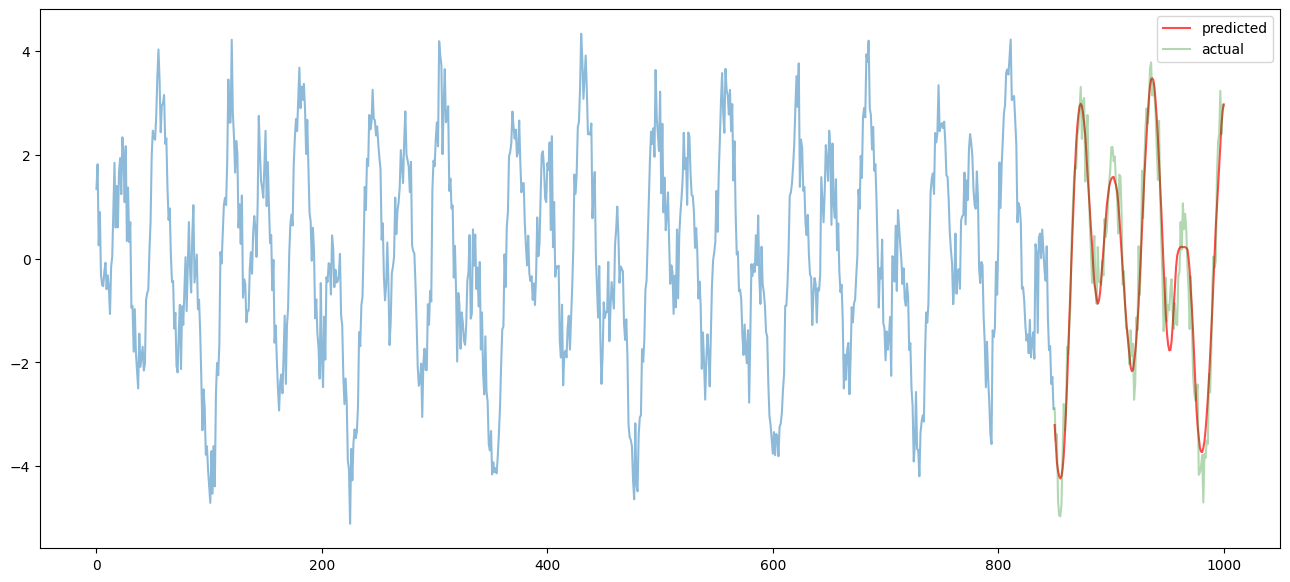
\includegraphics[width=\textwidth]{LSTM-prediction.png}
	\caption{Прогноз с использованием LSTM}
	\label{fig:fig1}
\end{figure}

Ряд восстанавливается неплохо, однако минусом является то, что при усложнении данных сильно растёт сложность модели. Так же, LSTM не может работать с многомерными рядами.

\subsection{SARIMA}

ARIMA позволяет находить авторегрессионные зависимости. SARIMA (Seasonal ARIMA) учитывает так же сезонность данных. Это может быть полезным в случае с данными природного характера, как например, температура воздуха или выработка электричества.

\begin{figure}
	\centering
	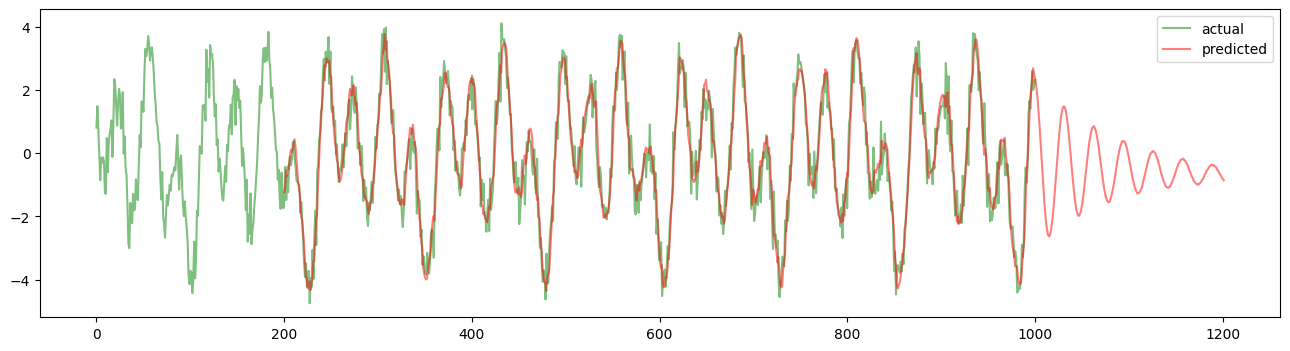
\includegraphics[width=\textwidth]{SARIMA-prediction.png}
	\caption{Прогноз с использованием SARIMA}
	\label{fig:fig2}
\end{figure}

Ряд прогнозируется довольно плохо, в случае если он имеет достаточно нетривиальную структуру. Так же, в данных может не быть явной сезонности, что ухудшает точность данного метода.

\subsection{MSSA}

MSSA (Multivariate Singular Spectrum Analysis) в отличие от других методов позволяет брать во внимание корреляцию между несколькими рядами и прогнозировать несколько.

% \section{Headings: first level}
% \label{sec:headings}

% \lipsum[4] See Section \ref{sec:headings}.

% \subsection{Headings: second level}
% \lipsum[5]
% \begin{equation}
% 	\xi _{ij}(t)=P(x_{t}=i,x_{t+1}=j|y,v,w;\theta)= {\frac {\alpha _{i}(t)a^{w_t}_{ij}\beta _{j}(t+1)b^{v_{t+1}}_{j}(y_{t+1})}{\sum _{i=1}^{N} \sum _{j=1}^{N} \alpha _{i}(t)a^{w_t}_{ij}\beta _{j}(t+1)b^{v_{t+1}}_{j}(y_{t+1})}}
% \end{equation}

% \subsubsection{Headings: third level}
% \lipsum[6]

% \paragraph{Paragraph}
% \lipsum[7]



% \section{Examples of citations, figures, tables, references}
% \label{sec:others}

% \subsection{Citations}
% Citations use \verb+natbib+. The documentation may be found at
% \begin{center}
% 	\url{http://mirrors.ctan.org/macros/latex/contrib/natbib/natnotes.pdf}
% \end{center}

% Here is an example usage of the two main commands (\verb+citet+ and \verb+citep+): Some people thought a thing \citep{kour2014real, hadash2018estimate} but other people thought something else \citep{kour2014fast}. Many people have speculated that if we knew exactly why \citet{kour2014fast} thought this\dots

% \subsection{Figures}
% \lipsum0]
% See Figure \ref{fig:fig1}. Here is how you add footnotes. \footnote{Sample of the first footnote.}
% \lipsum[11]

% \begin{figure}
% 	\centering
% 	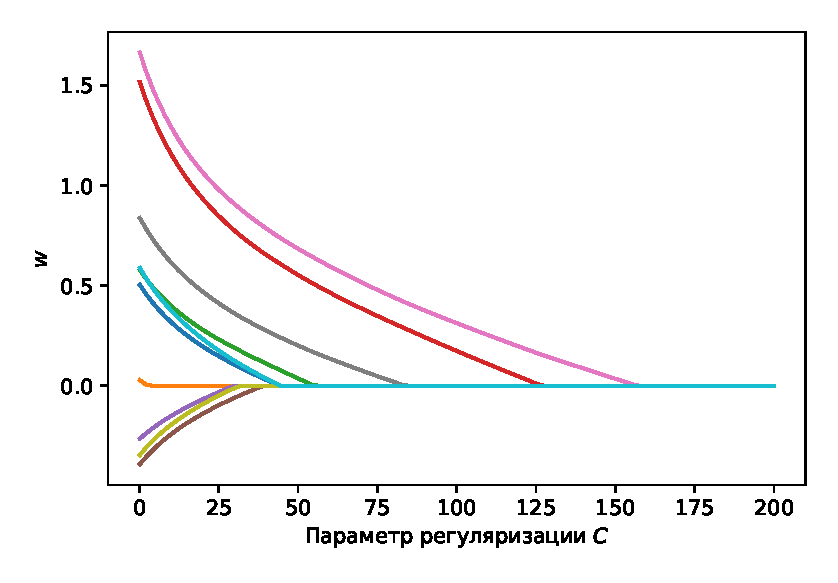
\includegraphics[width=0.5\textwidth]{../figures/log_reg_cs_exp.eps}
% 	\caption{Sample figure caption.}
% 	\label{fig:fig1}
% \end{figure}

% \subsection{Tables}
% See awesome Table~\ref{tab:table}.

% The documentation for \verb+booktabs+ (`Publication quality tables in LaTeX') is available from:
% \begin{center}
% 	\url{https://www.ctan.org/pkg/booktabs}
% \end{center}


% \begin{table}
% 	\caption{Sample table title}
% 	\centering
% 	\begin{tabular}{lll}
% 		\toprule
% 		\multicolumn{2}{c}{Part}                   \\
% 		\cmidrule(r){1-2}
% 		Name     & Description     & Size ($\mu$m) \\
% 		\midrule
% 		Dendrite & Input terminal  & $\sim$100     \\
% 		Axon     & Output terminal & $\sim$10      \\
% 		Soma     & Cell body       & up to $10^6$  \\
% 		\bottomrule
% 	\end{tabular}
% 	\label{tab:table}
% \end{table}

% \subsection{Lists}
% \begin{itemize}
% 	\item Lorem ipsum dolor sit amet
% 	\item consectetur adipiscing elit.
% 	\item Aliquam dignissim blandit est, in dictum tortor gravida eget. In ac rutrum magna.
% \end{itemize}



\bibliography{references}
\bibliographystyle{plain}


\end{document}